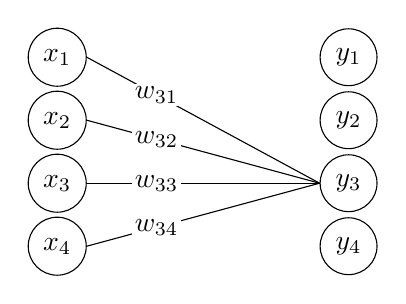
\begin{tikzpicture}
  \foreach \i/\y in {1/3.8, 2/3.0, 3/2.2, 4/1.4} {
    \node[draw, rounded corners=0.1pt, shape=circle] (x\i) at (0,\y) {$x_\i$};
    \node[draw, rounded corners=0.1pt, shape=circle] (y\i) at (3.7,\y) {$y_\i$};
  }

  \foreach \j in {1,...,4} {
    \draw (x\j.east) -- node[pos=0.3, fill=white, inner sep=1pt] {$w_{3\j}$} (y3.west);
  }
\end{tikzpicture}
